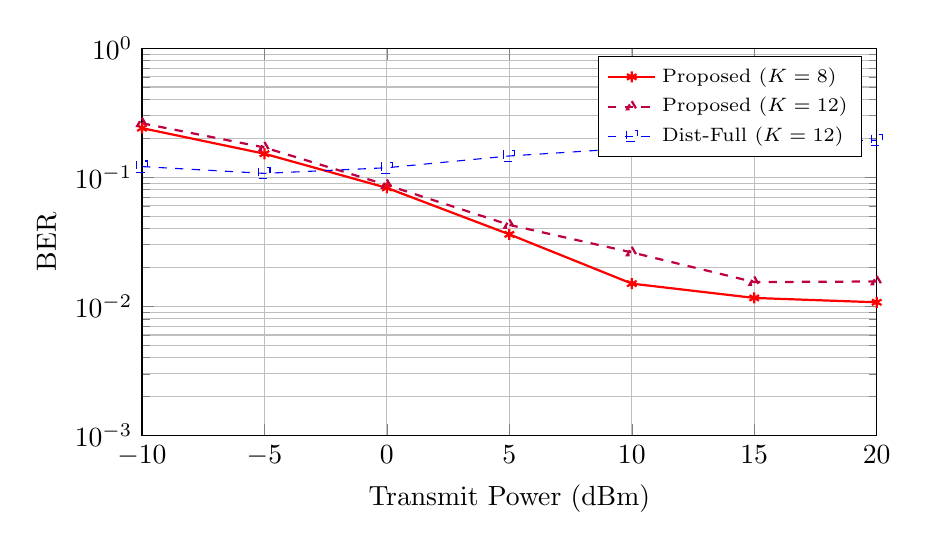
\begin{tikzpicture}
\begin{semilogyaxis}[
    width=0.9\linewidth,
    height=6.5cm,
    xlabel={Transmit Power (dBm)},
    ylabel={BER},
    xmin=-10, xmax=20,
    ymin=1e-3, ymax=1,
    grid=both,
    legend style={at={(0.98,0.98)},anchor=north east,font=\scriptsize},
    legend cell align={left}
]
\addplot[color=red,mark=asterisk,thick] coordinates {
(-10, 0.24025) (-5, 0.15213) (0, 0.08275) (5, 0.03612) (10, 0.01500) (15, 0.01162) (20, 0.01075)
};
\addlegendentry{Proposed ($K=8$)}

\addplot[color=purple,mark=triangle,thick,dashed] coordinates {
(-10, 0.26192) (-5, 0.17008) (0, 0.08708) (5, 0.04275) (10, 0.02617) (15, 0.01542) (20, 0.01558)
};
\addlegendentry{Proposed ($K=12$)}

\addplot[color=blue,mark=square,dashed] coordinates {
(-10, 0.12100) (-5, 0.10717) (0, 0.11850) (5, 0.14617) (10, 0.16800) (15, 0.18683) (20, 0.19375)
};
\addlegendentry{Dist-Full ($K=12$)}
\end{semilogyaxis}
\end{tikzpicture}